\section{HIRS SRF Data Plots}
%============================
\label{app.srf_data_plots}

\subsection{Channel 1}
%---------------------

\begin{figure}[H]
  \centering
  \begin{tabular}{c c}
    \includegraphics[scale=0.3]{graphics/srf/hirs2_tirosn-1.eps} &
    \includegraphics[scale=0.3]{graphics/tfit/hirs2_tirosn-1.tfit.eps} \\
    \includegraphics[scale=0.3]{graphics/srf/hirs2_n10-1.eps} &
    \includegraphics[scale=0.3]{graphics/tfit/hirs2_n10-1.tfit.eps} \\
    \includegraphics[scale=0.3]{graphics/srf/hirs3_n16-1.eps} &
    \includegraphics[scale=0.3]{graphics/tfit/hirs3_n16-1.tfit.eps}
  \end{tabular}
  \caption{HIRS channel 1 spectral responses (left panels) and polychromatic correction temperature fit residuals (right panels) for TIROS-N to NOAA-10 (top), NOAA-10 to NOAA-16 (middle) and NOAA-16 to MetOp-B (bottom). Vertical dashed lines in the SRF plots are the locations of the computed central frequencies.}
  \label{fig:srf_tfit_ch1}
\end{figure}

\subsection{Channel 2}
%---------------------

\begin{figure}[H]
  \centering
  \begin{tabular}{c c}
    \includegraphics[scale=0.3]{graphics/srf/hirs2_tirosn-2.eps} &
    \includegraphics[scale=0.3]{graphics/tfit/hirs2_tirosn-2.tfit.eps} \\
    \includegraphics[scale=0.3]{graphics/srf/hirs2_n10-2.eps} &
    \includegraphics[scale=0.3]{graphics/tfit/hirs2_n10-2.tfit.eps} \\
    \includegraphics[scale=0.3]{graphics/srf/hirs3_n16-2.eps} &
    \includegraphics[scale=0.3]{graphics/tfit/hirs3_n16-2.tfit.eps}
  \end{tabular}
  \caption{HIRS channel 2 spectral responses (left panels) and polychromatic correction temperature fit residuals (right panels) for TIROS-N to NOAA-10 (top), NOAA-10 to NOAA-16 (middle) and NOAA-16 to MetOp-B (bottom). Vertical dashed lines in the SRF plots are the locations of the computed central frequencies.}
  \label{fig:srf_tfit_ch2}
\end{figure}

\subsection{Channel 3}
%---------------------

\begin{figure}[H]
  \centering
  \begin{tabular}{c c}
    \includegraphics[scale=0.3]{graphics/srf/hirs2_tirosn-3.eps} &
    \includegraphics[scale=0.3]{graphics/tfit/hirs2_tirosn-3.tfit.eps} \\
    \includegraphics[scale=0.3]{graphics/srf/hirs2_n10-3.eps} &
    \includegraphics[scale=0.3]{graphics/tfit/hirs2_n10-3.tfit.eps} \\
    \includegraphics[scale=0.3]{graphics/srf/hirs3_n16-3.eps} &
    \includegraphics[scale=0.3]{graphics/tfit/hirs3_n16-3.tfit.eps}
  \end{tabular}
  \caption{HIRS channel 3 spectral responses (left panels) and polychromatic correction temperature fit residuals (right panels) for TIROS-N to NOAA-10 (top), NOAA-10 to NOAA-16 (middle) and NOAA-16 to MetOp-B (bottom). Vertical dashed lines in the SRF plots are the locations of the computed central frequencies.}
  \label{fig:srf_tfit_ch3}
\end{figure}

\subsection{Channel 4}
%---------------------

\begin{figure}[H]
  \centering
  \begin{tabular}{c c}
    \includegraphics[scale=0.3]{graphics/srf/hirs2_tirosn-4.eps} &
    \includegraphics[scale=0.3]{graphics/tfit/hirs2_tirosn-4.tfit.eps} \\
    \includegraphics[scale=0.3]{graphics/srf/hirs2_n10-4.eps} &
    \includegraphics[scale=0.3]{graphics/tfit/hirs2_n10-4.tfit.eps} \\
    \includegraphics[scale=0.3]{graphics/srf/hirs3_n16-4.eps} &
    \includegraphics[scale=0.3]{graphics/tfit/hirs3_n16-4.tfit.eps}
  \end{tabular}
  \caption{HIRS channel 4 spectral responses (left panels) and polychromatic correction temperature fit residuals (right panels) for TIROS-N to NOAA-10 (top), NOAA-10 to NOAA-16 (middle) and NOAA-16 to MetOp-B (bottom). Vertical dashed lines in the SRF plots are the locations of the computed central frequencies.}
  \label{fig:srf_tfit_ch4}
\end{figure}

\subsection{Channel 5}
%---------------------

\begin{figure}[H]
  \centering
  \begin{tabular}{c c}
    \includegraphics[scale=0.3]{graphics/srf/hirs2_tirosn-5.eps} &
    \includegraphics[scale=0.3]{graphics/tfit/hirs2_tirosn-5.tfit.eps} \\
    \includegraphics[scale=0.3]{graphics/srf/hirs2_n10-5.eps} &
    \includegraphics[scale=0.3]{graphics/tfit/hirs2_n10-5.tfit.eps} \\
    \includegraphics[scale=0.3]{graphics/srf/hirs3_n16-5.eps} &
    \includegraphics[scale=0.3]{graphics/tfit/hirs3_n16-5.tfit.eps}
  \end{tabular}
  \caption{HIRS channel 5 spectral responses (left panels) and polychromatic correction temperature fit residuals (right panels) for TIROS-N to NOAA-10 (top), NOAA-10 to NOAA-16 (middle) and NOAA-16 to MetOp-B (bottom). Vertical dashed lines in the SRF plots are the locations of the computed central frequencies.}
  \label{fig:srf_tfit_ch5}
\end{figure}

\subsection{Channel 6}
%---------------------

\begin{figure}[H]
  \centering
  \begin{tabular}{c c}
    \includegraphics[scale=0.3]{graphics/srf/hirs2_tirosn-6.eps} &
    \includegraphics[scale=0.3]{graphics/tfit/hirs2_tirosn-6.tfit.eps} \\
    \includegraphics[scale=0.3]{graphics/srf/hirs2_n10-6.eps} &
    \includegraphics[scale=0.3]{graphics/tfit/hirs2_n10-6.tfit.eps} \\
    \includegraphics[scale=0.3]{graphics/srf/hirs3_n16-6.eps} &
    \includegraphics[scale=0.3]{graphics/tfit/hirs3_n16-6.tfit.eps}
  \end{tabular}
  \caption{HIRS channel 6 spectral responses (left panels) and polychromatic correction temperature fit residuals (right panels) for TIROS-N to NOAA-10 (top), NOAA-10 to NOAA-16 (middle) and NOAA-16 to MetOp-B (bottom). Vertical dashed lines in the SRF plots are the locations of the computed central frequencies.}
  \label{fig:srf_tfit_ch6}
\end{figure}

\subsection{Channel 7}
%---------------------

\begin{figure}[H]
  \centering
  \begin{tabular}{c c}
    \includegraphics[scale=0.3]{graphics/srf/hirs2_tirosn-7.eps} &
    \includegraphics[scale=0.3]{graphics/tfit/hirs2_tirosn-7.tfit.eps} \\
    \includegraphics[scale=0.3]{graphics/srf/hirs2_n10-7.eps} &
    \includegraphics[scale=0.3]{graphics/tfit/hirs2_n10-7.tfit.eps} \\
    \includegraphics[scale=0.3]{graphics/srf/hirs3_n16-7.eps} &
    \includegraphics[scale=0.3]{graphics/tfit/hirs3_n16-7.tfit.eps}
  \end{tabular}
  \caption{HIRS channel 7 spectral responses (left panels) and polychromatic correction temperature fit residuals (right panels) for TIROS-N to NOAA-10 (top), NOAA-10 to NOAA-16 (middle) and NOAA-16 to MetOp-B (bottom). Vertical dashed lines in the SRF plots are the locations of the computed central frequencies.}
  \label{fig:srf_tfit_ch7}
\end{figure}

\subsection{Channel 8}
%---------------------

\begin{figure}[H]
  \centering
  \begin{tabular}{c c}
    \includegraphics[scale=0.3]{graphics/srf/hirs2_tirosn-8.eps} &
    \includegraphics[scale=0.3]{graphics/tfit/hirs2_tirosn-8.tfit.eps} \\
    \includegraphics[scale=0.3]{graphics/srf/hirs2_n10-8.eps} &
    \includegraphics[scale=0.3]{graphics/tfit/hirs2_n10-8.tfit.eps} \\
    \includegraphics[scale=0.3]{graphics/srf/hirs3_n16-8.eps} &
    \includegraphics[scale=0.3]{graphics/tfit/hirs3_n16-8.tfit.eps}
  \end{tabular}
  \caption{HIRS channel 8 spectral responses (left panels) and polychromatic correction temperature fit residuals (right panels) for TIROS-N to NOAA-10 (top), NOAA-10 to NOAA-16 (middle) and NOAA-16 to MetOp-B (bottom). Vertical dashed lines in the SRF plots are the locations of the computed central frequencies.}
  \label{fig:srf_tfit_ch8}
\end{figure}

\subsection{Channel 9}
%---------------------

\begin{figure}[H]
  \centering
  \begin{tabular}{c c}
    \includegraphics[scale=0.3]{graphics/srf/hirs2_tirosn-9.eps} &
    \includegraphics[scale=0.3]{graphics/tfit/hirs2_tirosn-9.tfit.eps} \\
    \includegraphics[scale=0.3]{graphics/srf/hirs2_n10-9.eps} &
    \includegraphics[scale=0.3]{graphics/tfit/hirs2_n10-9.tfit.eps} \\
    \includegraphics[scale=0.3]{graphics/srf/hirs3_n16-9.eps} &
    \includegraphics[scale=0.3]{graphics/tfit/hirs3_n16-9.tfit.eps}
  \end{tabular}
  \caption{HIRS channel 9 spectral responses (left panels) and polychromatic correction temperature fit residuals (right panels) for TIROS-N to NOAA-10 (top), NOAA-10 to NOAA-16 (middle) and NOAA-16 to MetOp-B (bottom). Vertical dashed lines in the SRF plots are the locations of the computed central frequencies.}
  \label{fig:srf_tfit_ch9}
\end{figure}

\subsection{Channel 10}
%---------------------

\begin{figure}[H]
  \centering
  \begin{tabular}{c c}
    \includegraphics[scale=0.3]{graphics/srf/hirs2_tirosn-10.eps} &
    \includegraphics[scale=0.3]{graphics/tfit/hirs2_tirosn-10.tfit.eps} \\
    \includegraphics[scale=0.3]{graphics/srf/hirs2_n10-10.eps} &
    \includegraphics[scale=0.3]{graphics/tfit/hirs2_n10-10.tfit.eps} \\
    \includegraphics[scale=0.3]{graphics/srf/hirs3_n16-10.eps} &
    \includegraphics[scale=0.3]{graphics/tfit/hirs3_n16-10.tfit.eps}
  \end{tabular}
  \caption{HIRS channel 10 spectral responses (left panels) and polychromatic correction temperature fit residuals (right panels) for TIROS-N to NOAA-10 (top), NOAA-10 to NOAA-16 (middle) and NOAA-16 to MetOp-B (bottom). Vertical dashed lines in the SRF plots are the locations of the computed central frequencies.}
  \label{fig:srf_tfit_ch10}
\end{figure}

\subsection{Channel 11}
%---------------------

\begin{figure}[H]
  \centering
  \begin{tabular}{c c}
    \includegraphics[scale=0.3]{graphics/srf/hirs2_tirosn-11.eps} &
    \includegraphics[scale=0.3]{graphics/tfit/hirs2_tirosn-11.tfit.eps} \\
    \includegraphics[scale=0.3]{graphics/srf/hirs2_n10-11.eps} &
    \includegraphics[scale=0.3]{graphics/tfit/hirs2_n10-11.tfit.eps} \\
    \includegraphics[scale=0.3]{graphics/srf/hirs3_n16-11.eps} &
    \includegraphics[scale=0.3]{graphics/tfit/hirs3_n16-11.tfit.eps}
  \end{tabular}
  \caption{HIRS channel 11 spectral responses (left panels) and polychromatic correction temperature fit residuals (right panels) for TIROS-N to NOAA-10 (top), NOAA-10 to NOAA-16 (middle) and NOAA-16 to MetOp-B (bottom). Vertical dashed lines in the SRF plots are the locations of the computed central frequencies.}
  \label{fig:srf_tfit_ch11}
\end{figure}

\subsection{Channel 12}
%---------------------

\begin{figure}[H]
  \centering
  \begin{tabular}{c c}
    \includegraphics[scale=0.3]{graphics/srf/hirs2_tirosn-12.eps} &
    \includegraphics[scale=0.3]{graphics/tfit/hirs2_tirosn-12.tfit.eps} \\
    \includegraphics[scale=0.3]{graphics/srf/hirs2_n10-12.eps} &
    \includegraphics[scale=0.3]{graphics/tfit/hirs2_n10-12.tfit.eps} \\
    \includegraphics[scale=0.3]{graphics/srf/hirs3_n16-12.eps} &
    \includegraphics[scale=0.3]{graphics/tfit/hirs3_n16-12.tfit.eps}
  \end{tabular}
  \caption{HIRS channel 12 spectral responses (left panels) and polychromatic correction temperature fit residuals (right panels) for TIROS-N to NOAA-10 (top), NOAA-10 to NOAA-16 (middle) and NOAA-16 to MetOp-B (bottom). Vertical dashed lines in the SRF plots are the locations of the computed central frequencies.}
  \label{fig:srf_tfit_ch12}
\end{figure}

\subsection{Channel 13}
%---------------------

\begin{figure}[H]
  \centering
  \begin{tabular}{c c}
    \includegraphics[scale=0.3]{graphics/srf/hirs2_tirosn-13.eps} &
    \includegraphics[scale=0.3]{graphics/tfit/hirs2_tirosn-13.tfit.eps} \\
    \includegraphics[scale=0.3]{graphics/srf/hirs2_n10-13.eps} &
    \includegraphics[scale=0.3]{graphics/tfit/hirs2_n10-13.tfit.eps} \\
    \includegraphics[scale=0.3]{graphics/srf/hirs3_n16-13.eps} &
    \includegraphics[scale=0.3]{graphics/tfit/hirs3_n16-13.tfit.eps}
  \end{tabular}
  \caption{HIRS channel 13 spectral responses (left panels) and polychromatic correction temperature fit residuals (right panels) for TIROS-N to NOAA-10 (top), NOAA-10 to NOAA-16 (middle) and NOAA-16 to MetOp-B (bottom). Vertical dashed lines in the SRF plots are the locations of the computed central frequencies.}
  \label{fig:srf_tfit_ch13}
\end{figure}

\subsection{Channel 14}
%---------------------

\begin{figure}[H]
  \centering
  \begin{tabular}{c c}
    \includegraphics[scale=0.3]{graphics/srf/hirs2_tirosn-14.eps} &
    \includegraphics[scale=0.3]{graphics/tfit/hirs2_tirosn-14.tfit.eps} \\
    \includegraphics[scale=0.3]{graphics/srf/hirs2_n10-14.eps} &
    \includegraphics[scale=0.3]{graphics/tfit/hirs2_n10-14.tfit.eps} \\
    \includegraphics[scale=0.3]{graphics/srf/hirs3_n16-14.eps} &
    \includegraphics[scale=0.3]{graphics/tfit/hirs3_n16-14.tfit.eps}
  \end{tabular}
  \caption{HIRS channel 14 spectral responses (left panels) and polychromatic correction temperature fit residuals (right panels) for TIROS-N to NOAA-10 (top), NOAA-10 to NOAA-16 (middle) and NOAA-16 to MetOp-B (bottom). Vertical dashed lines in the SRF plots are the locations of the computed central frequencies.}
  \label{fig:srf_tfit_ch14}
\end{figure}

\subsection{Channel 15}
%---------------------

\begin{figure}[H]
  \centering
  \begin{tabular}{c c}
    \includegraphics[scale=0.3]{graphics/srf/hirs2_tirosn-15.eps} &
    \includegraphics[scale=0.3]{graphics/tfit/hirs2_tirosn-15.tfit.eps} \\
    \includegraphics[scale=0.3]{graphics/srf/hirs2_n10-15.eps} &
    \includegraphics[scale=0.3]{graphics/tfit/hirs2_n10-15.tfit.eps} \\
    \includegraphics[scale=0.3]{graphics/srf/hirs3_n16-15.eps} &
    \includegraphics[scale=0.3]{graphics/tfit/hirs3_n16-15.tfit.eps}
  \end{tabular}
  \caption{HIRS channel 15 spectral responses (left panels) and polychromatic correction temperature fit residuals (right panels) for TIROS-N to NOAA-10 (top), NOAA-10 to NOAA-16 (middle) and NOAA-16 to MetOp-B (bottom). Vertical dashed lines in the SRF plots are the locations of the computed central frequencies.}
  \label{fig:srf_tfit_ch15}
\end{figure}

\subsection{Channel 16}
%---------------------

\begin{figure}[H]
  \centering
  \begin{tabular}{c c}
    \includegraphics[scale=0.3]{graphics/srf/hirs2_tirosn-16.eps} &
    \includegraphics[scale=0.3]{graphics/tfit/hirs2_tirosn-16.tfit.eps} \\
    \includegraphics[scale=0.3]{graphics/srf/hirs2_n10-16.eps} &
    \includegraphics[scale=0.3]{graphics/tfit/hirs2_n10-16.tfit.eps} \\
    \includegraphics[scale=0.3]{graphics/srf/hirs3_n16-16.eps} &
    \includegraphics[scale=0.3]{graphics/tfit/hirs3_n16-16.tfit.eps}
  \end{tabular}
  \caption{HIRS channel 16 spectral responses (left panels) and polychromatic correction temperature fit residuals (right panels) for TIROS-N to NOAA-10 (top), NOAA-10 to NOAA-16 (middle) and NOAA-16 to MetOp-B (bottom). Vertical dashed lines in the SRF plots are the locations of the computed central frequencies.}
  \label{fig:srf_tfit_ch16}
\end{figure}

\subsection{Channel 17}
%---------------------

\begin{figure}[H]
  \centering
  \begin{tabular}{c c}
    \includegraphics[scale=0.3]{graphics/srf/hirs2_tirosn-17.eps} &
    \includegraphics[scale=0.3]{graphics/tfit/hirs2_tirosn-17.tfit.eps} \\
    \includegraphics[scale=0.3]{graphics/srf/hirs2_n10-17.eps} &
    \includegraphics[scale=0.3]{graphics/tfit/hirs2_n10-17.tfit.eps} \\
    \includegraphics[scale=0.3]{graphics/srf/hirs3_n16-17.eps} &
    \includegraphics[scale=0.3]{graphics/tfit/hirs3_n16-17.tfit.eps}
  \end{tabular}
  \caption{HIRS channel 17 spectral responses (left panels) and polychromatic correction temperature fit residuals (right panels) for TIROS-N to NOAA-10 (top), NOAA-10 to NOAA-16 (middle) and NOAA-16 to MetOp-B (bottom). Vertical dashed lines in the SRF plots are the locations of the computed central frequencies.}
  \label{fig:srf_tfit_ch17}
\end{figure}

\subsection{Channel 18}
%---------------------

\begin{figure}[H]
  \centering
  \begin{tabular}{c c}
    \includegraphics[scale=0.3]{graphics/srf/hirs2_tirosn-18.eps} &
    \includegraphics[scale=0.3]{graphics/tfit/hirs2_tirosn-18.tfit.eps} \\
    \includegraphics[scale=0.3]{graphics/srf/hirs2_n10-18.eps} &
    \includegraphics[scale=0.3]{graphics/tfit/hirs2_n10-18.tfit.eps} \\
    \includegraphics[scale=0.3]{graphics/srf/hirs3_n16-18.eps} &
    \includegraphics[scale=0.3]{graphics/tfit/hirs3_n16-18.tfit.eps}
  \end{tabular}
  \caption{HIRS channel 18 spectral responses (left panels) and polychromatic correction temperature fit residuals (right panels) for TIROS-N to NOAA-10 (top), NOAA-10 to NOAA-16 (middle) and NOAA-16 to MetOp-B (bottom). Vertical dashed lines in the SRF plots are the locations of the computed central frequencies.}
  \label{fig:srf_tfit_ch18}
\end{figure}

\subsection{Channel 19}
%---------------------

\begin{figure}[H]
  \centering
  \begin{tabular}{c c}
    \includegraphics[scale=0.3]{graphics/srf/hirs2_tirosn-19.eps} &
    \includegraphics[scale=0.3]{graphics/tfit/hirs2_tirosn-19.tfit.eps} \\
    \includegraphics[scale=0.3]{graphics/srf/hirs2_n10-19.eps} &
    \includegraphics[scale=0.3]{graphics/tfit/hirs2_n10-19.tfit.eps} \\
    \includegraphics[scale=0.3]{graphics/srf/hirs3_n16-19.eps} &
    \includegraphics[scale=0.3]{graphics/tfit/hirs3_n16-19.tfit.eps}
  \end{tabular}
  \caption{HIRS channel 19 spectral responses (left panels) and polychromatic correction temperature fit residuals (right panels) for TIROS-N to NOAA-10 (top), NOAA-10 to NOAA-16 (middle) and NOAA-16 to MetOp-B (bottom). Vertical dashed lines in the SRF plots are the locations of the computed central frequencies.}
  \label{fig:srf_tfit_ch19}
\end{figure}

